

\question(20分){已知控制系统结构图如下所示,已知 $G(s)=\frac{1}{s(s+1)^2}$, 非线性环节描述函数 $N_1(A)=\frac{k_1}{A},N_2(A)=\frac{k_2}{A},(A>1)$,求使系统稳定无自振的$k_1,k_2$范围。
	
	
	\begin{tikzpicture}[node distance=3em,auto,>=latex', thick]
	%\path[use as bounding box] (-1,0) rectangle (10,-2); 
	\tikzstyle{block} = [draw,rectangle,thick,minimum height=1em,minimum width=1em]
	\tikzstyle{sum} = [draw,circle,inner sep=0mm,minimum size=2mm]
	\tikzstyle{branch} = [circle,fill,inner sep=0pt,minimum size=1mm]
	\tikzstyle{connector} = [->,thick]
	
	\def\r{\node(r){$r(t)$};}
	\def\n{\node(n){$n(t)$};}
	\def\b(#1){\node[branch](b#1){};}
	\def\p(#1){\node[sum](p#1){};}
	\def\gc{\node[block](gc){$N_2(A)$};}
	\def\gr{\node[block](gr){$N_1(A)$};}
	\def\gn{\node[block](gn){$G_n(s)$};}
	\def\gp{\node[block](gp){$G(s)$};}
	\def\g(#1){\node[block](g#1){$1$};}
	\def\c{\node(c){$c(t)$};}
	
	\matrix[ampersand replacement=\&, row sep=1em, column sep=2em]{
		\&          \&     \& \gr    \&       \&         \\
		\r  \&    \p(e) \& \b(r)  \& \gc \&  \p(r) \& \gp \& \b(c)  \& \c  \\
		\&         \&         \& \g(h)    \\
	};
	\draw [connector](r) -- (pe) ; 
	\draw [connector](br) |- (gr) ; 
	\draw [connector](gr) -| (pr) ;
	\draw [connector](pe) -- (gc) ; 
	\draw [connector](gc) -- (pr) ; 
	\draw [connector](pr) -- (gp) ; 
	\draw [connector](gp) -- (c) ; 
	\draw [connector](bc) |- (gh) ; 
	\draw [connector](gh) -| node[near end , left]{$-$} (pe) ; 
	\end{tikzpicture} 
	
	\onlyanswer{
		答:
		两个非线性环节并联,其描述函数为两个环节描述函数之和。
		\begin{align*}
		N(A) &= N_1(A)+N_2(A) \\
		&= \frac{k_1}{A}+\frac{k_2}{A}\\
		-\frac{1}{N(A)}&=-\frac{A}{k_1+k_2}\\
		\angle G(j\omega) &=-90^\circ-2\angle(s+1)\\
		\angle G(j\omega)|_{\omega=1} &= -180^\circ\\
		G(j\omega)|_{\omega=1}&=-0.5
		\end{align*}
		
			\begin{tikzpicture}[scale=1]
			\coordinate (o) at (0,0);
			\coordinate (ox) at (2,0);
			\draw[->] (-2,0) -- (ox);
			\draw[->] (0,-1) -- (0,1);
			\draw[->,violet,thick] (-1,0) -- (-2,0); % -1/N(A)=-A/(k_1+k_2)
			\draw (-1,0) node[pin=100:$-\frac{1}{k_1+k_2}$] {};
			\draw (-1,0) node [red,thick,circle,fill,inner sep=0pt,minimum size=1mm] {};
			\draw [red,thick,smooth] plot coordinates {(-1.5,-2)(-1,-0.5)(-0.5,0)(-0.2,0.1) (0,0) }; %G(s)=1/s/(1+s)^2
			\draw[->,red,dashed,thick] (2,0) arc (0:-100:2.5);
			\draw (0,1) node[left] {$j$};
			\end{tikzpicture}
			
		当 $-\frac{1}{N(A)}<-0.5$ 时,系统稳定无自振,得:
		\begin{align*}
		-\frac{A}{k_1+k_2} &< -0.5 \\
		0<k_1+k_2&<2A\\
		0<k_1+k_2&<2
		\end{align*}
		
	}
}





\question(20分){单位负反馈控制系统开环传递函数:
	$$G(s)=\frac{10}{s(10s+1)}$$
	串联校正网络:
	$$G_c(s)=k\cdot\frac{10 s+1}{a s+1}$$
	求解参数 $k,a$ 使校正后系统截止频率不变,相角裕度为 $45^\circ$ 。
	
	\onlyanswer
	{
		答:
		计算校正前截止频率:
		\begin{align*}
		|G(s)| &=1 \\
		\omega_c &=1
		\end{align*}
		根据相角裕度要求,得:
		\begin{align*}
		\angle (a j+1)&=45^{\circ} \\
		a &=1
		\end{align*}
		校正后前截止频率不变:
		\begin{align*}
		|G_c(\omega_c)G(\omega_c)| &=1 \\
		k &\approx 0.1
		\end{align*}
	}
}




\question(20分){已知控制系统结构图如下所示,已知 $$G(s)=\frac{1}{s},G_c(s)=1,G_r(s)=\frac{k_1 s}{T_1s+1},G_n(s)=\frac{k_2 s}{T_2s+1},(T_1\geq 0,T_2\geq 0)$$
当$r(t)=t,n(t)=1,(t>0)$时, 是否存在 $k_1,k_2$ 使稳态误差为零?
	当$r(t)=sin(t),n(t)=sin(2t),(t>0)$ 时,是否存在 $k_1\geq 0,k_2\geq 0,T_1\geq 0,T_2\geq 0 $ 使系统稳态输出 $c(t)$ 满足$|c(t)-sin(t)|<0.01 $ ?
	
	
	\begin{tikzpicture}[node distance=3em,auto,>=latex', thick]
	%\path[use as bounding box] (-1,0) rectangle (10,-2); 
	\tikzstyle{block} = [draw,rectangle,thick,minimum height=1em,minimum width=1em]
	\tikzstyle{sum} = [draw,circle,inner sep=0mm,minimum size=2mm]
	\tikzstyle{branch} = [circle,fill,inner sep=0pt,minimum size=1mm]
	\tikzstyle{connector} = [->,thick]
	
	\def\r{\node(r){$r(t)$};}
	\def\n{\node(n){$n(t)$};}
	\def\b(#1){\node[branch](b#1){};}
	\def\p(#1){\node[sum](p#1){};}
	\def\gc{\node[block](gc){$G_c(s)$};}
	\def\gr{\node[block](gr){$G_r(s)$};}
	\def\gn{\node[block](gn){$G_n(s)$};}
	\def\gp{\node[block](gp){$G(s)$};}
	\def\g(#1){\node[block](g#1){$1$};}
	\def\c{\node(c){$c(t)$};}
	
	\matrix[ampersand replacement=\&, row sep=1em, column sep=2em]{
		\&          \&        \&     \&       \&        \&    \& \n \\
		\\
		\&          \&   \gr  \&     \&       \&        \& \gn \\
		\r  \&   \b(r)  \& \p(e)  \& \gc \& \p(r) \&  \p(n) \& \gp \& \p(c) \& \b(c)  \& \c  \\
		\&         \&         \& \g(h)    \\
	};
	\draw [connector](r) -- (pe) ; 
	\draw [connector](n) -- (pc) ; 
	\draw [connector](n) |- (gn) ; 
	\draw [connector](br) |- (gr) ; 
	\draw [connector](gr) -| (pr) ;
	\draw [connector](gn) -| (pn) ; 
	\draw [connector](pe) -- node[midway]{$E(s)$} (gc) ; 
	\draw [connector](gc) -- (pr) ; 
	\draw [connector](pr) -- (pn) ; 
	\draw [connector](pn) -- (gp) ; 
	\draw [connector](gp) -- (pc) ; 
	\draw [connector](pc) -- (c) ; 
	\draw [connector](bc) |- (gh) ; 
	\draw [connector](gh) -| node[near end , left]{$-$} (pe) ; 
	\end{tikzpicture} 
	
	\onlyanswer
	{
		答:
		
		\begin{align*}
		E(s)&=\frac{1-G_r(s)G(s)}{1+G_c(s)G(s)}R(S)-\frac{1+G_n(s)G(s)}{1+G_c(s)G(s)}N(s)\\
		&=\frac{1-\frac{k_1s}{(T_1s+1)s}}{1+\frac{1}{s}}\cdot\frac{1}{s^2}-\frac{1+\frac{k_2s}{(T_2s+1)s}}{1+\frac{1}{s}}\cdot\frac{1}{s}\\
		&=\frac{T_1s+1-k_1}{(T_1s+1)(s+1)s}-\frac{T_2s+1+k_2}{(T_2s+1)(s+1)}\\
		\end{align*}
		当 $k_1=1$ 时,
		\begin{align*}
		sE(s)&=\frac{T_1s}{(T_1s+1)(s+1)}-\frac{s(T_2s+1+k_2)}{(T_2s+1)(s+1)}\\
		\lim_{s\to 0}sE(s)&=0
		\end{align*}
		系统稳态时,输出可由频域模型求解:
		\begin{align*}
		e(t)&=c(t)-r(t)\\
		&=c(t)-sin(t)\\
		E(j\omega)&=\frac{1-\frac{k_1j\omega}{(T_1j\omega+1)j\omega}}{1+\frac{1}{j\omega}}R(j\omega)-\frac{1+\frac{k_2j\omega}{(T_2j\omega+1)j\omega}}{1+\frac{1}{j\omega}} N(j\omega)\\
		&=\frac{j\omega(T_1j\omega+1-k_1)}{(T_1j\omega+1)(j\omega+1)}R(j\omega)-\frac{j\omega(T_2j\omega+1+k_2)}{(T_2j\omega+1)(j\omega+1)}N(j\omega)
		\end{align*}
		
		
		为满足 $r(t)=sin(t),n(t)=sin(2t)$ 时,$ |c(t)-sin(t)|<0.01$ 要求
		
		 $$\left.\frac{E(j\omega)}{R(j\omega)}\right|_{\omega=1}<0.01,\left.\frac{E(j\omega)}{R(j\omega)}\right|_{\omega=2}<0.01$$
		
		但与$k_1\geq 0, k_2\geq 0$ 矛盾,因此不存在满足要求的 $k_1,k_2$。
		
		
		若不限制 $k_2\geq 0$ , 当 $k_1=1,k_2=-1$ 时
		\begin{align*}
		E(j\omega)&=\frac{-T_1\omega^2}{(T_1j\omega+1)(j\omega+1)}R(j\omega)+\frac{T_2\omega^2}{(T_2j\omega+1)(j\omega+1)}N(j\omega)\\
		\end{align*}
		$r(t)=sin(t),n(t)=sin(2t)$ 时,
		\begin{align*}
		|c(t)-sin(t)|&=|e(t)|\\
		&\leq \left|\left.\frac{-T_1\omega^2}{(T_1j\omega+1)(j\omega+1)}\right|_{\omega=1}+\left.\frac{T_2\omega^2}{(T_2j\omega+1)(j\omega+1)}\right|_{\omega=2}\right| \\
		&\leq \left|\frac{-T_1}{(T_1j+1)(j+1)}\right|+\left|\frac{4T_2}{(2T_2j+1)(2j+1)}\right|
		\end{align*}
		选取 $T_1<<1,T_2<<1$ ,得: $|c(t)-sin(t)|\approx 0$,满足 $|c(t)-sin(t)|<0.01$
		
	}
}


\question(20分) { 已知控制系统结构图如下所示,求 $E_1(z),E_2(z)$ ;为使系统稳定,应如何选取 $k$ ?

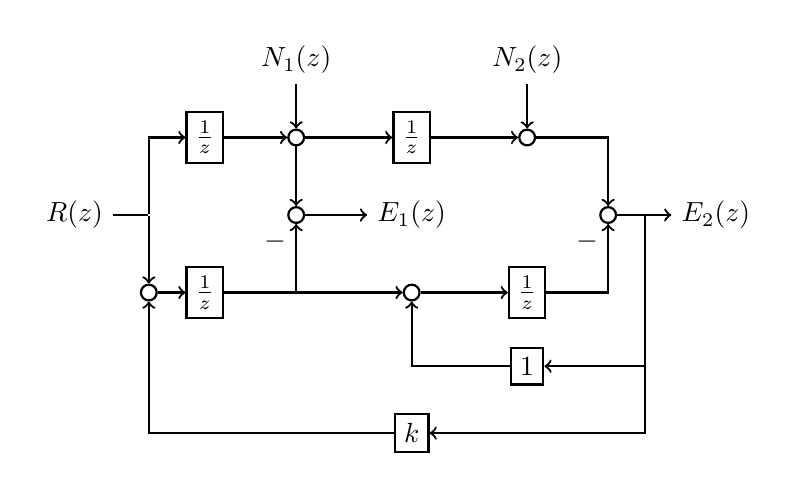
\begin{tikzpicture}[scale=1, thick] 
\tikzstyle{block} = [draw,rectangle,thick,minimum height=1em,minimum width=1em]
\tikzstyle{sum} = [draw,circle,inner sep=0mm,minimum size=2mm]
\tikzstyle{branch} = [inner sep=0pt,minimum size=0pt]
\tikzstyle{connector} = [->,thick]
\matrix[ampersand replacement=\&, row sep=1em, column sep=1em]{
	\&  \&  \& \node(n1){$N_1(z)$};\&\&\node(n2){$N_2(z)$}; \\
	
	\&  \&  \node[block](g1){$\frac{1}{z}$}; \& \node[sum](p1) {}; \& \node[block] (g2){$\frac{1}{z}$}; \& \node[sum](p2) {};  \\
	
	\node[] (r) {$R(z)$}; \& 
	\node[branch] (b1) {} ; \&
	\&
	\node[sum](p3) {}; \&
	\node[] (e1) {$E_1(z)$} ; \&
	\&
	\node[sum](p4) {};\&
	\node[branch] (b2) {} ;  \&
	\node[] (e2) {$E_2(z)$} ; 
	\\
	
	\& \node[sum](p5) {}; \&  \node[block](g3){$\frac{1}{z}$}; \&  \&
	\node[sum](p6) {}; \& \node[block](g4){$\frac{1}{z}$};   \\
	\& \& \& \& \& \node[block](h1){$1$}; \\
	\& \& \& \& \node[block](h2){$k$}; \\
};
\draw [connector] (n1) -- (p1);
\draw [connector] (n2) -- (p2);
\draw [thick] (r) -- (b1);
\draw [connector] (b1) |- (g1);
\draw [connector] (b1) -- (p5);
\draw [connector] (p5) -- (g3);
\draw [connector] (g1) -- (p1);
\draw [connector] (p1) -- (g2);\draw [connector] (p1) -- (p3);
\draw [connector] (g3) -- (p6);
\draw [connector] (p6) -- (g4);
\draw [connector] (g3) -|  node[very near end,left] {$ - $} (p3);
\draw [connector] (p3) -- (e1);
\draw [connector] (g2) -- (p2);
\draw [connector] (p2) -| (p4);
\draw [connector] (g4) -| node[very near end,left] {$ - $} (p4);
\draw [connector] (p4) -- (e2);
\draw [connector] (b2) |- (h1);
\draw [connector] (b2) |- (h2);
\draw [connector] (h1) -|  node[very near end,left] {$ $} (p6);
\draw [connector] (h2) -|  node[very near end,left] {$ $} (p5);
\end{tikzpicture} 



\onlyanswer
{
	解:
	
	根据结构图可得:
	\begin{align*}
		E_1(z) &=R(z)z^{-1}+N_1(z) -R(z)z^{-1}-E_2(z)kz^{-1} \\
		E_2(z )&=R(z)z^{-2}+N_2(z)+N_1(z)z^{-1} -R(z)z^{-2}-E_2(z)kz^{-2}-E_2(z)z^{-1} 
	\end{align*}
	化简得:
	\begin{align*}
	E_2(z )&=N_2(z)+N_1(z)z^{-1}-E_2(z)kz^{-2}-E_2(z)z^{-1}\\
	       &=\frac{N_2(z)+N_1(z)z^{-1}}{1+kz^{-2}+z^{-1}}\\
	       &=\frac{z^2 N_2(z)+z N_1(z)}{z^2+z+k}\\
	E_1(z) &=N_1(z)-E_2(z)kz^{-1} \\
	       &=N_1(z)-\frac{kz N_2(z)+k N_1(z)}{z^2+z+k}\\
	       &=\frac{(z^2+z)N_1(z)-kz N_2(z)}{z^2+z+k}\\
	\end{align*}
	
	利用 $w$ 变换分析稳定性:
		\begin{align*}
		\left(\frac{w+1}{w-1}\right)^2+\frac{w+1}{w-1}+k &=0 \\
		(w+1)^2+(w+1)(w-1)+k(w-1)^2 &=0   \\
		(2+k)w^2+(2-2k)w+k &=0
		\end{align*}
		当 $0<k<1$ 时系统稳定。
		
	
}

}

%\onlytest{\vskip 3em}

%\onlytest{\newpage}


\question(20分) { 已知控制系统结构图如下所示, 分析使系统稳定的 $k_1,k_2$ 取值范围;若 $k_1=1$, 是否存在 $k_2$ 使 $e(nT)=0$ ?

\begin{tikzpicture}[node distance=3em,auto,>=latex', thick]
%\path[use as bounding box] (-1,0) rectangle (10,-2); 
\tikzstyle{block} = [draw,rectangle,thick,minimum height=1em,minimum width=1em]
\tikzstyle{sum} = [draw,circle,inner sep=0mm,minimum size=2mm]
\tikzstyle{branch} = [circle,fill,inner sep=0pt,minimum size=1mm]
\tikzstyle{connector} = [->,thick]

\def\r{\node(r){$r(t)$};}
\def\rd{\node(rd){$r^*(t)$};}
\def\b(#1){\node[branch](b#1){};}
\def\p(#1){\node[sum](p#1){};}
\def\s(#1){\path[->] node[minimum size=2em] (s#1) {}; \draw (s#1.west)--(s#1.north east);\draw[->] (s#1.north west) arc (70:0:1.7em);\draw (s#1.south) node {$T$};}
\def\sd(#1){\path[->] node[minimum size=2em] (sd#1) {}; \draw[dashed] (sd#1.west)--(sd#1.north east);\draw[dashed,->] (sd#1.north west) arc (70:0:1.7em);\draw[dashed] (sd#1.south) node {$T$};}
\def\gc{\node[block](gc){$\dfrac{k_1}{s}$};}
\def\gd{\node[block](gd){$\dfrac{k_2}{s}$};}
\def\gh0{\node[block](gh0){$\dfrac{1-e^{-sT}}{s}$};}
\def\g(#1){\node[block](g#1){$1$};}
\def\ed{\node(ed){$e^*(t)$};}

\matrix[ampersand replacement=\&, row sep=1em, column sep=2em]{
	\&    \&        \& \g(ch)    \\
	\&    \p(ce) \&  \& \gc  \& \& \b(c)  \\
	\r  \&   \b(r)  \&   \&   \&   \& \p(e)   \&  \s(e)  \& \ed  \\
	\&  \p(de) \& \s(de)  \& \gh0 \& \gd  \& \b(d)    \\  
	\&         \&   \& \g(dh)    \\
};
\draw [connector](br) -- (pce) ; 
\draw [connector](r) -| (pde) ; 
\draw [connector](pce) -- (gc) ; 
\draw [connector](gc) -| (pe) ; 
\draw [connector](bc) |- (gch) ; 
\draw [connector](gch) -| node[near end , left]{$-$} (pce) ; 
\draw [](pde) -- (sde) ;
\draw [connector](sde) -- (gh0) ;  
\draw [connector](gh0) -- (gd) ;  
\draw [connector](gd) -| node[near end , left ]{$-$} (pe) ; 
\draw [connector](bd) |- (gdh) ; 
\draw [connector](gdh) -| node[near end , left ]{$-$} (pde) ; 
\draw [](pe)  -- (se) ; 
\draw [connector](se) -- (ed) ; 
\end{tikzpicture} 


常见 $Z$ 变换表:
$$
\begin{array}{ccc}
f(t)     &   F(s)  &  F(Z)   \\ 
\delta(t)   &   1      &  1    \\  
1(t)         &   \frac{1}{s} &  \frac{1}{1-z^{-1}}   \\ 
t            &   \frac{1}{s^2} &  \frac{Tz^{-1}}{(1-z^{-1})^2}   \\  
e^{-at}      &   \frac{1}{s+a} &  \frac{1}{1-e^{-aT}z^{-1}}  \\ 
a^{t/T}      &   \frac{1}{s-(1/T)\ln a} & \frac{1}{1-az^{-1}} 
\end{array}
$$

\onlyanswer
{
	答:由结构图可知:
	\begin{align*}
	R(s) &= \frac{1}{s} \\
	E^*(s) &= \left[\frac{\frac{k_1}{s}}{1+\frac{k_1}{s}}R(s)\right]^*-\frac{[\frac{k_2}{s}]^*}{1+[\frac{k_2}{s}]^*}R^*(s) \\
	&= \left[\frac{k_1}{s(s+k_1)}\right]^* -\frac{[\frac{(1-e^{-sT})k_2}{s^2}]^*}{1+[\frac{(1-e^{-sT})k_2}{s^2}]^*}R^*(s) \\
	&= \left[\frac{1}{s}-\frac{1}{s+k_1}\right]^* -\frac{[\frac{(1-e^{-sT})k_2}{s^2}]^*}{1+[\frac{(1-e^{-sT})k_2}{s^2}]^*}R^*(s) \\
	E(z)  &=\frac{1}{1-z^{-1}}-\frac{1}{1-e^{-k_1T}z^{-1}}-\frac{\frac{(1-z^{-1})k_2Tz^{-1}}{(1-z^{-1})^2}}{1+\frac{(1-z^{-1})k_2Tz^{-1}}{(1-z^{-1})^2}}\frac{1}{1-z^{-1}} \\
	&=\frac{1}{1-z^{-1}}-\frac{1}{1-e^{-k_1T}z^{-1}}-\frac{k_2Tz^{-1}}{1-z^{-1}+k_2 T z^{-1}}\frac{1}{1-z^{-1}} \\
	&=\frac{1}{1-z^{-1}}-\frac{1}{1-e^{-k_1T}z^{-1}}-\frac{1}{1-z^{-1}}+\frac{1}{1-z^{-1}+k_2Tz^{-1}} \\
	&=-\frac{1}{1-e^{-k_1T}z^{-1}}+\frac{1}{1-z^{-1}+k_2Tz^{-1}} \\
	e(nT) &=-e^{-nk_1T}+(1-k_2T)^n
	\end{align*}
	由 $e(nT)$ 表达式可知,当 $k_1\in(0,\infty),k_2\in(0,\frac{2}{T})$ 时系统稳定。当 $k_2=\frac{1-e^{-k_1T}}{T}$ 时,$e(nT)=0$ 。
}

}

